\chapter{Vocabulaire utile}

Avant de commencer, il est important de comprendre certaines notions utiles :

\paragraph{}
Le \textbf{\textit{deep learning}} est une méthode d’apprentissage automatique basée sur une
modélisation de type neuronal. Ainsi, un algorithme utilisant le \textit{deep learning}
apprend par lui-même et devient de plus en plus performant au fur et à mesure qu’il accumule
les exemples. Il suffit de lui spécifier les paramètres du problème qu’il doit résoudre et de
lui donner des exemples sur lesquels s’entraîner.

\paragraph{}
Une \textbf{base d’apprentissage} (ou base d'entraînement) est un ensemble d’exemples
que l’on fournit à un algorithme de \textit{deep learning} afin que celui-ci puisse apprendre
sur ces exemples.

\paragraph{}
La \textbf{vérité terrain} est, dans le cas de notre projet, un ensemble de documents manuscrits
annotés de diverses informations telles que la position des paragraphes dans les documents ou encore la
transcription informatique des textes. Cette vérité a été établie au préalable par des humains et non
de manière automatique.

\paragraph{}
Un \textbf{polygone concave} est un polygone complexe dont l’intérieur est un ensemble concave.
D'une manière géométrique, on dit qu'un polygone est concave si lorsque l'on trace une droite passant
par l’un de ses côtés, alors le polygone se retrouve en partie coupé par cette droite.
Un polygone non concave est dit convexe.

\paragraph{}
\begin{mdframed}[frametitle={Figure 1 : Exemples de polygones concave (à gauche) et convexe (à droite)}, innerbottommargin=10]
\begin{center}
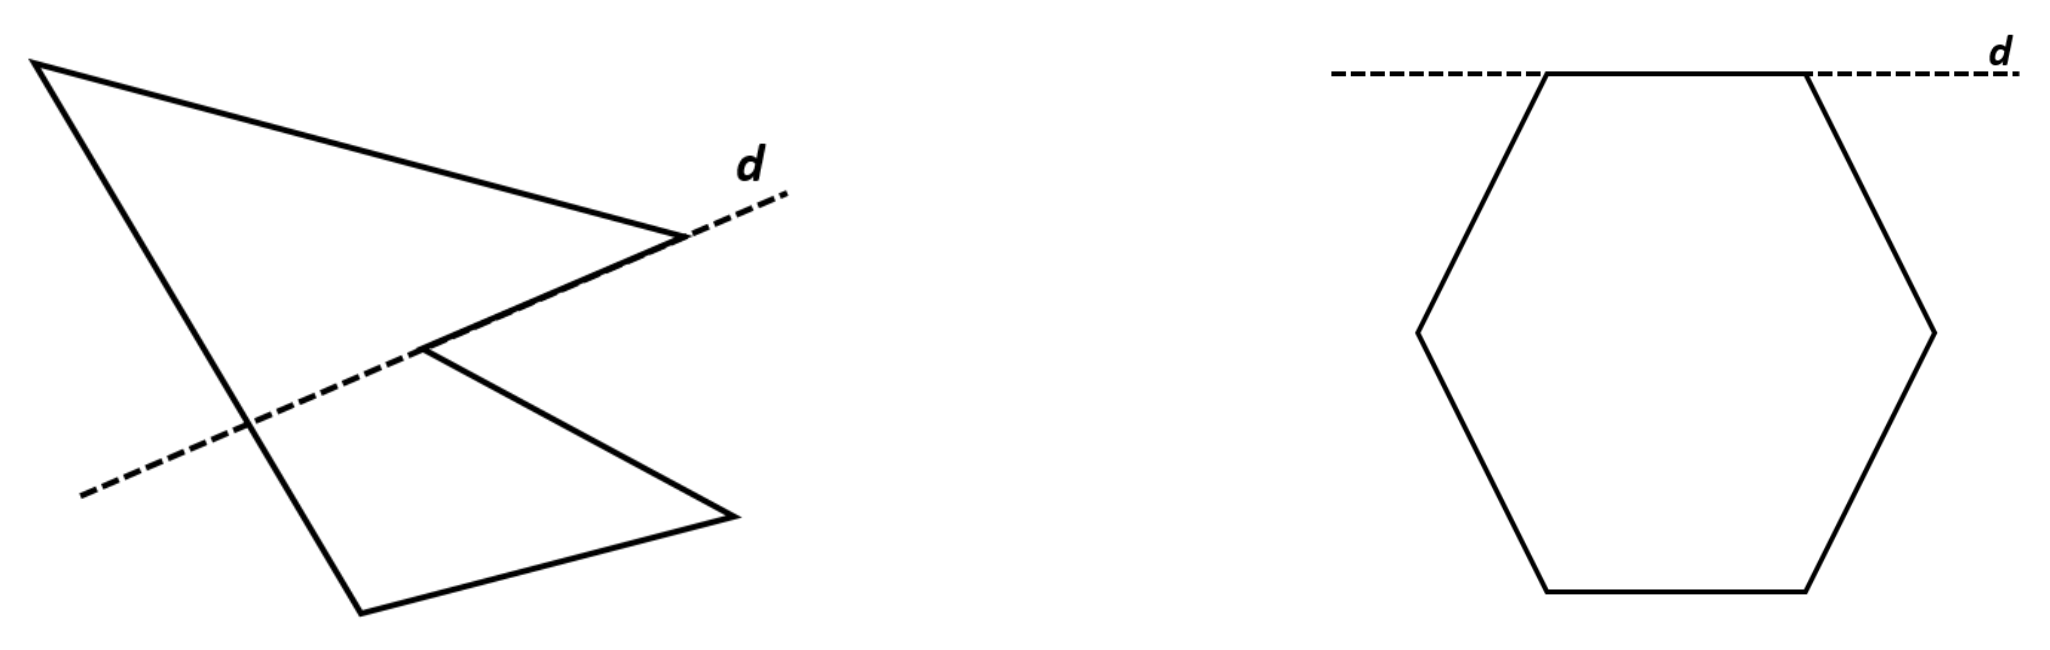
\includegraphics[width=\linewidth]{polygone.png}
\end{center}
\end{mdframed}

\paragraph{}
Une \textbf{imagette} est une image réduite d'une autre image. Dans le cas de notre projet,
cela correspond à une partie de texte manuscrit découpée à partir du document initial.

\paragraph{}
Nous appellerons \textbf{retranscription} la transcription informatique d’un texte manuscrit.